% Условная компиляция для самостоятельной работы
\ifdefined\mainfile
    % Если это часть основного файла, не добавляем начало и конец документа
\else
    \documentclass[12pt, a4paper]{report}
    \usepackage{/Users/vladbelousov/Desktop/Semestr_4-FP-NSU/Настройка/library}
    \usepackage[utf8]{inputenc} % Подключение поддержки UTF-8
    \begin{document}
\fi

%%-------------------------------%%

\chapter{Геометрия пространств со скалярным произведением.}

\section{Линейные пространства}

\begin{center}
    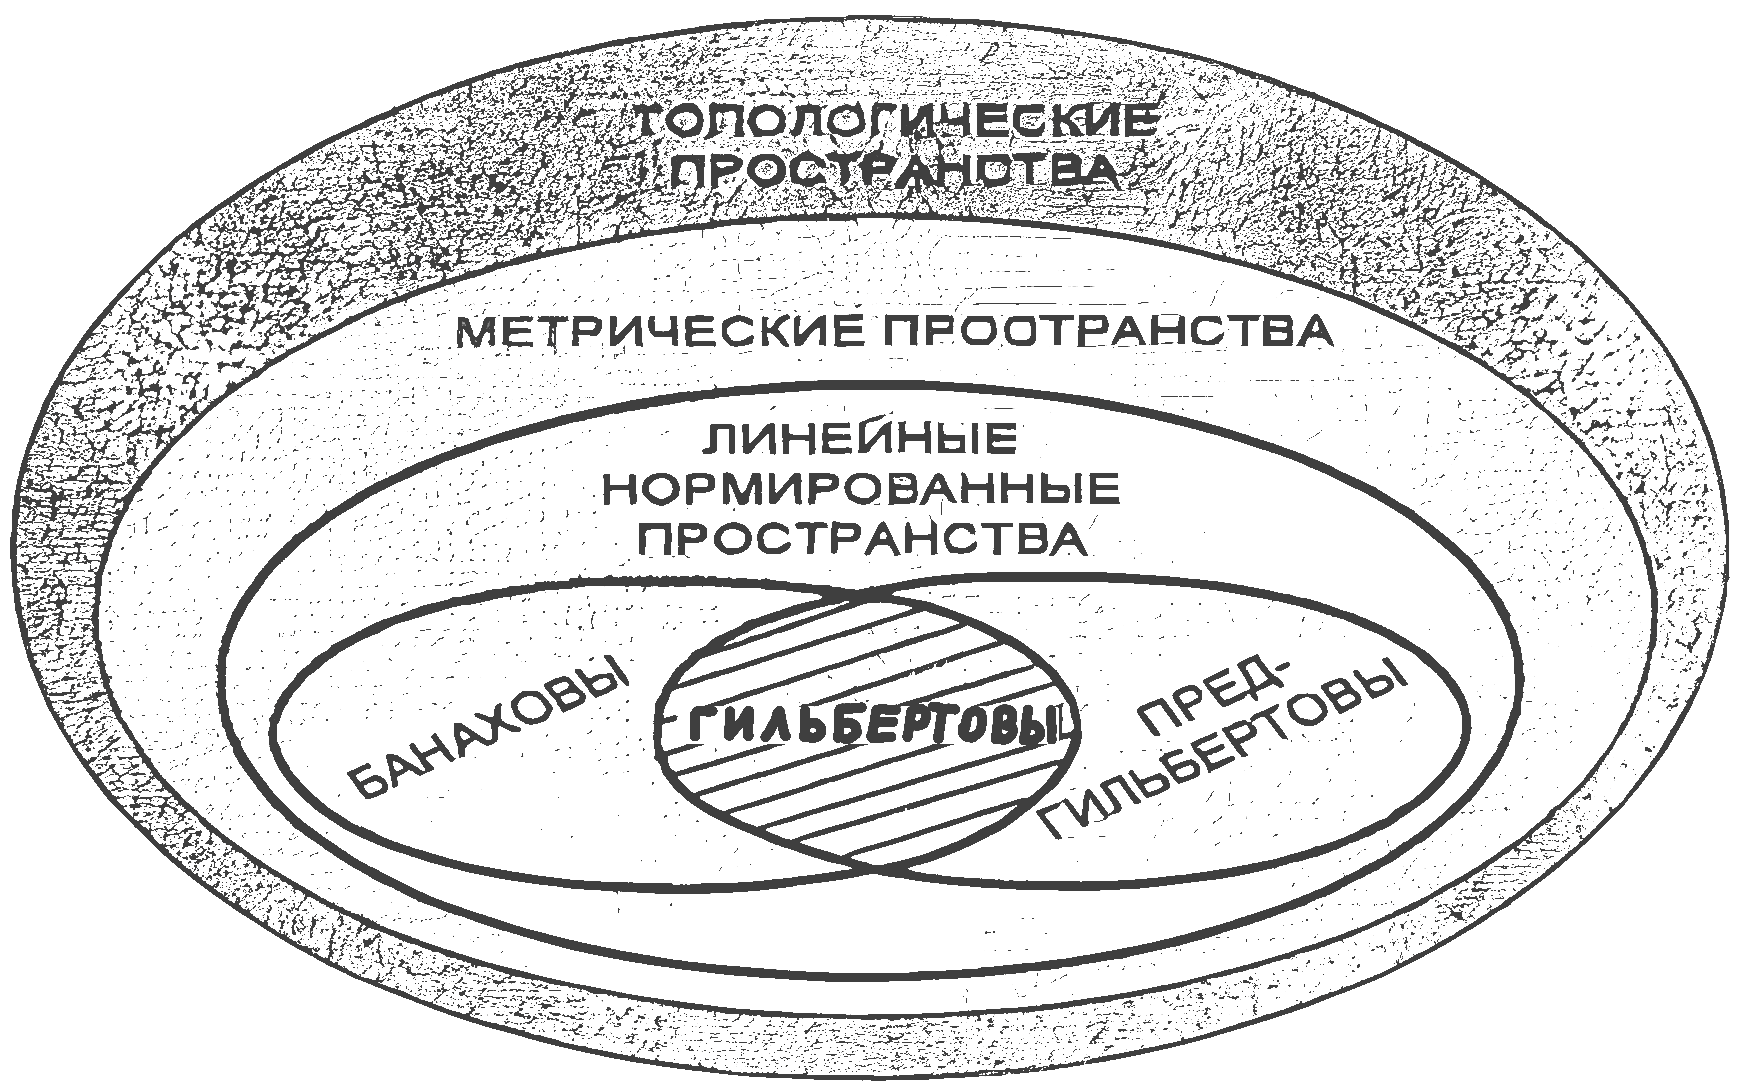
\includegraphics[width=0.5\textwidth]{/Users/vladbelousov/Desktop/Semestr_4-FP-NSU/ОФА/Лекции_по_дням/image/1.png}
\end{center}

\begin{definition}[Метрическое прострнвство]
    Метрика \( \rho (x,y): M ^2 \to  \mathbb{R} \) 

    1) \( \forall x,y :\rho (x,y ) \geq 0 - ( \rho(x,y) = 0 \Leftrightarrow x=y)   \) 

    2) \( \forall x,y \in  M :\rho(x,y )= \rho (y,x)  \)
    
    3) \( \forall x,y,z :\rho(x,z) \le  \rho(x,y)+\rho(y,z) \)
\end{definition}

\( B_{\varepsilon}(x) = \{ y \in  M | \rho(x,y) < \varepsilon \} \) 

\begin{definition}
    Множество открытое, если любая точка в нем содержится в нем вместе некоторой окрестностью.
\end{definition}

Пример дискреткой метрики: 

\[ 
\rho(x,y) = 
\begin{cases} 
    1 \quad x \neq y \\
    0 \quad  x=y   
\end{cases} 
\] 

\section{Линейно (векторное) пространство}

\begin{definition}
    Непустое множество элементов L произвольной природы, называется линейным (векторным) над полем чисел \( \mathbb{R} (\mathbb{C})\) если 

    1) \( \forall x,y   \) введена операция сложения:

    \( \quad  \) 1.1)  \( x+y = y+x \) (коммутативность)
    
    \( \quad  \) 1.2) \( x+(y+z)= (x+y ) +z \) (ассоциативность)
    
    \( \quad  \) 1.3) В L существует элемент называемым нулем 0: \( x+0 = x \text{ }  , \forall x \in  L \)  

    \( \quad  \) 1.4) \( \forall x \in  L \)  существует противоположный элемент принадлежащий 
    
    L: \( x+y = 0 \) , обозначается как \( -x \)

    2) \( \forall x \in  L \)  и \( \forall  \) числа \( \alpha \in  \mathbb{R}(\mathbb{C}) \) определен вектор из L - произведения элементов на число \( \alpha , \alpha x \in  L \):
    
    \( \quad  \) 1.1) \( \alpha (\beta x )= (\alpha \beta )x  , \forall  \alpha, \beta  \)
    
    \( \quad  \) 1.2) \( 1 \cdot x =x  \) (существования единицы)
    
    \( \quad  \) 1.3) \( \alpha (x+y) = \alpha x + \alpha y \)

    \( \quad  \) 1.4) \( (\alpha + \beta )x = \alpha x + \beta x \) 


\end{definition}

Примеры: 

1)
\[ \begin{aligned}
\begin{array}{ll}
    \mathbb{R}^{n }\\
    \mathbb{C}^{n}  
\end{array}
\begin{array}{ll}
    \quad \alpha(x_1,x_2, \ldots, x_n) \\
    + \\
    \quad \beta (y_1,y_2, \ldots ,y_n )
\end{array}
\quad =(\alpha x_1 + \beta y_1 ,\dots \alpha x_n + \beta y_n)
\end{aligned} \] 

2) \( C[a,b] = \{f(a,b) \to  \mathbb{C}, \text{ непрерывная функции } f \text{ - непрерывна }   \)\}

3) \(\displaystyle  L_p (x)= \{f \text{- измерима по Лебегу, заданная на } X , f: X \to  \mathbb{C} \text{ таких, что }   \)

\[  \int_{X}|f(x)|dx< \infty  \] 

4) \(\displaystyle  l_2 : x = \{x_1 , \ldots , x_n  \} \quad \sum ^{\infty }_{1}  |x_n| ^2 < \infty  \) 

\begin{definition}
    \( x_1, \ldots, x_n \)  называется линейно зависимыми, если \( \exists \alpha_1 , \ldots , \alpha _ n   \) не все равные нулю, такие что \( \alpha_1 x_1 + \dots + \alpha_n x_n=0   \)
    
    В противном случае: из того, что \( \alpha_1 x_1 + \dots + \alpha_n x_n=0 \) следует, что все \( \alpha_i =0  \) \( x_1, \ldots, x_n \)  называется линейно независимыми наборами  векторов.  
\end{definition}

\begin{definition}
    Бесконечный набор элементов L называется линейно независимым, если любой его конечный поднабор линейно независимым.
\end{definition}

\begin{definition}
    Если в L можно найти \( n  \)  линейно независимых векторов, а любой набор из \( n+1 \) векторов является линейно зависимыми, то \( \dim L= n \). Если в L можно указать   набор из произвольного числа линейно независимых элементов, то \( \dim L= \infty  \). 
\end{definition}

\begin{definition}
    Непустое подмножество \( S \subset L  \)  называется подпространством, если оно само является пространством введенных в L линейных операций.
\end{definition}

\begin{definition}
    Линейной  оболочкой  <M> называется совокупность всех линейных комбинаций  \( \alpha x + \beta y  \)  где \(  x,y \in  M  \subset \alpha, \beta \in  \mathbb{C}(\mathbb{R}) \) 

    <M> - подпространство в L  (натянутое или порожденное множеством элементов M)
\end{definition}

\section{Определение нормы} 

\begin{definition}
    Норма в линейном пространстве L:  \( \norm{\text{ } }  : L \to  \mathbb{R}^+ = [ 0 , \infty ) \)

    \( \forall x,y \in  L ,  \forall  \alpha \in  \mathbb{C}(\mathbb{R}) \) 
    
    1) \( ||x|| \geq  0 ,||x||=0 \Leftrightarrow x=0  \quad   \) (положительная определенность нормы)
    
    2) \( ||\alpha x||=|\alpha|||x || \quad  \)  (положительная однородность нормы) 

    3) \( ||x+y|| \le  ||x|+||y|| \)
\end{definition}

В конечномерных пространствах все нормы эквиваленты \( c_1||x||_1 \le  ||x||_2 \le  c_2 ||x||_1 \). В конечномерных пространствах это не так! 

Пример норм: 

\[1)  \norm{f}= \max _{t \in [ a,b]} |f(t)| \text{ - норма в }  C [ a,b]  \text{ равномерная норма.}  \] 

\[ \begin{aligned}
    2) &  \quad ||f||_{L_1} = \int_{X} |f|dx \text{ в  }  L_1 \\
    3) & \quad ||f||_{L_p} = \sqrt[p]{\int_{X}|f|^p dx} \text{в}  L_{p} \\
    4) & \quad ||x||_{l_2}= \sqrt{\sum^{\infty }_{i=1} |x_i| ^2   }   
\end{aligned} \] 

\begin{definition}
    Последовательность \( (x_n)_{n \in  N}  \) точек линейно нормированное пространств L сходятся к x, если  \( ||x_n - x|| \xrightarrow{n \to  \infty } 0 ,\forall \varepsilon > 0, \exists n_0, n > n_0 : ||x_n - x|| < \varepsilon   \) 
\end{definition}

\begin{definition}
    Предельной точкой \( M \subset L  \)  называется точка x, если существует сходящаяся к x последовательность элементов из M \( \exists x_n \in  M : x_n \to x  \) 
\end{definition}

\begin{definition}
    Замыканием \( \overline{M}  \) - объединение  M и его предельных точек (по конкретной норме). 
\end{definition}

\begin{definition}
    Множество замкнутое, если содержит все предельные точки.
\end{definition}

\begin{definition}
    Множество M в L - линейно нормированном пространстве называется плотным в L, если \( \overline{M}= L  \) 
\end{definition}

\begin{definition}
    Сепарабельное множество, если в нем \( \exists  \) счетное плотное подмножество
\end{definition}



%%-------------------------------%%

% Закрытие документа, если файл компилируется отдельно
\ifdefined\mainfile
    % Если это основной файл, не нужно заканчивать документ
\else
    \end{document}
\fi